\subsection{Budget-constrained investment (Experiment H)}
For the normal year, the deterministic optimum spends every budget level from 100 to 1{,}500~MEUR entirely on
PV: 126, 315, 629, 944, 1{,}258 and 1{,}888~MW. At 2{,}000~MEUR the PV bound (+2{,}000~MW) binds and the
budget does not. Neither wind nor storage enters at any budget. The budget shadow price falls from 0.070 to
0.024~EUR of annual saving per euro of capital as PV grows. These are diminishing but still positive returns,
and they are consistent with the PV marginal value of Experiment~J (140~kEUR/MW-yr against 80~kEUR/MW-yr of
annualised cost). The result reflects three assumptions: exports absorb midday surplus at 85\% of the import
price, there is no reserve requirement, and wind capacity factors are about 0.11 from coarse reanalysis.
Section~\ref{sec:sensitivity} tests the first of these.

\subsection{Deterministic versus stochastic planning (Experiment I)}
The two-stage programme has five scenarios, eight hourly weeks each, a 500~MEUR budget and CVaR at $\alpha=0.9$.
For every risk weight tested ($\lambda\in\{0,0.25,1,4\}$) it selects the \emph{same} portfolio as the
deterministic normal-year plan: +629~MW of PV, with no wind and no storage (Table~\ref{tab:risk-sweep}). The same
holds at a 1{,}500~MEUR budget. Each wait-and-see problem also chooses this plan, so the value of the stochastic
solution and the expected value of perfect information are both zero to solver precision
(Table~\ref{tab:stochastic}). CVaR$_{0.9}$ of operating cost is 397~MEUR/yr for both plans. Hypothesis~I is
therefore \textbf{not supported} under the base assumptions. PV is a \emph{no-regret} investment in every
scenario. Its value is set mainly by the import price, and it rises under stress. The budget binds before any
resource whose value depends on the scenario becomes competitive. The stochastic machinery still answers
question~6 of the study: under these assumptions, deterministic planning for an average year is not
penalised. One qualification matters. None of the five planning scenarios, the compound shock included
(70\% availability), reaches the import-availability regime of $\le$50\% in which shortages occur and
batteries become valuable (Sections~\ref{sec:results} and~\ref{sec:sensitivity}). A scenario set with even a
small probability of that regime could change the plan, and this is a priority for future work.

\IfFileExists{tables/tab_stochastic.tex}{\begin{table}[htbp]
\centering
\small
\caption{Two-stage stochastic versus deterministic planning (budget 500 MEUR, 8 representative weeks, water-value boundaries). E[cost]: expected total annualised cost (MEUR/yr) on all five scenarios; CVaR of operating cost (MEUR/yr). Risk-adjusted VSS = 0.00 MEUR/yr; EVPI is reported only for $\lambda=0$.}
\label{tab:stochastic}
\begin{adjustbox}{max width=\linewidth}
\begin{tabular}{lrrrrrr}
\toprule
Plan & +PV & +Wind & +B MW & +B MWh & E[cost] & CVaR$_{0.9}$ \\
\midrule
Stochastic (RP), $\lambda$=1 & 629 & 0 & 0 & 0 & 70.9 & 397.3 \\
Deterministic (normal year) & 629 & 0 & 0 & 0 & 70.9 & 397.3 \\
\bottomrule
\end{tabular}
\end{adjustbox}
\end{table}
}{}

\subsection{When does stochastic planning matter? (Experiment I2)}
To find the conditions under which uncertainty changes the decision, we repeated the comparison with export
capacity limited to 300~MW. Surplus PV must then be stored, absorbed by the reservoir or curtailed. We also
raised the budget, so that PV saturates before the budget binds (Table~\ref{tab:i2}). With 900~MW of export
capacity the stochastic and deterministic plans remain identical at every risk weight (VSS = 0). With
restricted exports and risk-neutral planning ($\lambda=0$), the stochastic plan adds slightly more PV than the
deterministic one (+26~MW at 1{,}000~MEUR, +75~MW at 1{,}500~MEUR), and the VSS is only 0.2--0.3~MEUR/yr. With
restricted exports, a 1{,}500~MEUR budget and $\lambda=1$, the decision changes qualitatively. The risk-averse
plan adds 1{,}520~MW of PV, 230~MW of \emph{wind} and a 30~MW / 66~MWh battery. The deterministic plan adds
1{,}232~MW of PV only. In the representative-week model the risk-averse plan raises expected cost by
7.8~MEUR/yr and lowers CVaR$_{0.9}$ of operating cost by 79~MEUR/yr (from 292 to 213); the risk-adjusted VSS is
71.5~MEUR/yr. Full-year chronological re-evaluation of the two plans confirms the trade-off. Expected total
cost is higher by 15.1~MEUR/yr (74.6 vs 59.5), CVaR$_{0.9}$ of operating cost is lower by 74.5~MEUR/yr (208.2
vs 282.7), and neither plan has any unserved energy. The hedge is mainly wind rather than storage. Once PV saturates
under the export limit, wind is the cheapest remaining way to cut imports in the high-price stress scenarios.
We did not decompose this mechanism further, for example by wind--PV correlation or season. Stochastic, risk-aware planning therefore matters when a no-regret resource
saturates because its surplus cannot leave the system. In that regime the choice among the remaining resources
depends on the tail scenarios.

\IfFileExists{tables/tab_i2.tex}{\begin{table}[htbp]
\centering
\scriptsize
\caption{Experiment I2: stochastic (RP) versus deterministic-plan evaluation (EEV) under restricted and full export capacity. Additions as PV/wind MW / battery MW/MWh; E = expected total annualised cost, CVaR$_{0.9}$ of operating cost and risk-adjusted VSS in MEUR/yr (representative weeks, water-value boundaries).}
\label{tab:i2}
\begin{adjustbox}{max width=\linewidth}
\begin{tabular}{lrrrrrrrrr}
\toprule
Export MW & Budget & $\lambda$ & Stoch. adds & Det. adds & E RP & E EEV & CVaR RP & CVaR EEV & VSS \\
\midrule
300 & 1\,000 & 0 & 1\,258/0/0/0 & 1\,232/0/0/0 & 62.0 & 62.1 & 288.1 & 292.0 & 0.2 \\
300 & 1\,000 & 1 & 1\,258/0/0/0 & 1\,232/0/0/0 & 62.0 & 62.1 & 288.1 & 292.0 & 4.1 \\
300 & 1\,500 & 0 & 1\,307/0/0/0 & 1\,232/0/0/0 & 61.8 & 62.1 & 281.1 & 292.0 & 0.3 \\
300 & 1\,500 & 1 & 1\,520/230/30/66 & 1\,232/0/0/0 & 70.0 & 62.1 & 212.7 & 292.0 & 71.5 \\
900 & 1\,500 & 0 & 1\,888/0/0/0 & 1\,888/0/0/0 & 12.9 & 12.9 & 170.2 & 170.2 & 0.0 \\
900 & 1\,500 & 1 & 1\,888/0/0/0 & 1\,888/0/0/0 & 12.9 & 12.9 & 170.2 & 170.2 & 0.0 \\
\bottomrule
\end{tabular}
\end{adjustbox}
\end{table}
}{}

\begin{figure}[htbp]
\centering
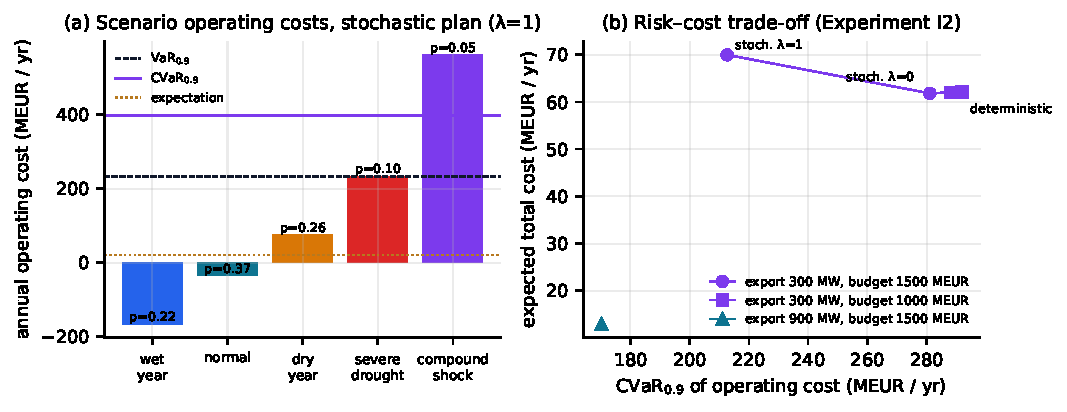
\includegraphics[width=\textwidth]{fig09_cvar.pdf}
\caption{(a) Annualised operating cost of the reference stochastic plan in each scenario, with probabilities, VaR$_{0.9}$,
CVaR$_{0.9}$ and the expectation. In the base case this plan is identical to the deterministic plan. (b) Expected total cost
versus CVaR$_{0.9}$ of operating cost for the deterministic plan and the stochastic plans ($\lambda=0,1$) in
Experiment~I2. Only with restricted exports and a large budget does risk aversion buy a material reduction in tail
cost.}
\label{fig:cvar}
\end{figure}


\subsection{Investment frontier}
Figure~\ref{fig:frontier} and Table~\ref{tab:strategies} compare the required strategies, the budget sweep and
the stochastic plans on equal terms, using the same representative-week evaluation. At 500~MEUR the strategies
rank as follows by expected total annualised cost: solar (70.9~MEUR/yr; identical to the coordinated and
climate-robust optima), baseline (109.4), wind (112.1) and battery-only (164.9). The battery-only plan has the
highest cost and the highest imports, because arbitrage increases gross imports. Across budgets, larger PV
additions lower both expected cost and imports. The non-dominated set in (expected cost, expected imports)
therefore collapses to the largest-PV plan, and the trade-off appears only in capital spent versus imports
(\texttt{pareto\_capex\_imports} in the artefact). We report this degenerate frontier as it is, rather than
constructing an artificial trade-off.

\begin{figure}[htbp]
\centering
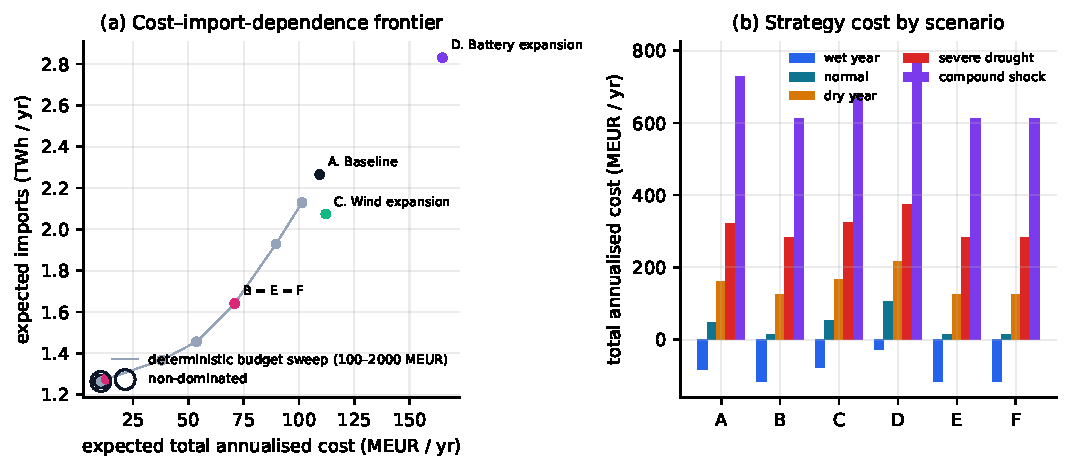
\includegraphics[width=\textwidth]{fig08_investment_frontier.pdf}
\caption{(a) Strategies in the plane of expected total annualised cost and expected imports, evaluated with the
same representative-week model over five scenarios. Outlined points are non-dominated. (b) Total annualised cost
of the required strategies A--F in each scenario.}
\label{fig:frontier}
\end{figure}

\begin{table}[htbp]
\centering
\scriptsize
\caption{Investment strategies evaluated on the five-scenario set (representative weeks, hourly). Additions in MW/MWh, overnight capex in MEUR, expected total annualised cost and severe-drought cost in MEUR/yr, expected imports in TWh/yr; ND marks the non-dominated set in (expected cost, expected imports).}
\label{tab:strategies}
\begin{tabular}{p{4.2cm}rrrrrrrrc}
\toprule
Strategy & +PV & +Wind & +B MW & +B MWh & Capex & E[cost] & E[imp.] & Cost sev. & ND \\
\midrule
A. Baseline & 0 & 0 & 0 & 0 & 0 & 109.4 & 2.27 & 320.4 &  \\
B. Solar expansion & 629 & 0 & 0 & 0 & 500 & 70.9 & 1.64 & 283.5 &  \\
C. Wind expansion & 0 & 418 & 0 & 0 & 500 & 112.1 & 2.07 & 323.7 &  \\
D. Battery expansion & 0 & 0 & 522 & 2\,087 & 500 & 164.9 & 2.83 & 373.4 &  \\
E. Coordinated (deterministic optimum) & 629 & 0 & 0 & 0 & 500 & 70.9 & 1.64 & 283.5 &  \\
F. Climate-robust (stochastic, CVaR λ=1) & 629 & 0 & 0 & 0 & 500 & 70.9 & 1.64 & 283.5 &  \\
Budget 100 MEUR (det.) & 126 & 0 & 0 & 0 & 100 & 101.4 & 2.13 & 312.9 &  \\
Budget 250 MEUR (det.) & 315 & 0 & 0 & 0 & 250 & 89.7 & 1.93 & 301.8 &  \\
Budget 750 MEUR (det.) & 944 & 0 & 0 & 0 & 750 & 53.7 & 1.46 & 266.5 &  \\
Budget 1000 MEUR (det.) & 1\,258 & 0 & 0 & 0 & 1\,000 & 37.9 & 1.37 & 251.2 &  \\
Budget 1500 MEUR (det.) & 1\,888 & 0 & 0 & 0 & 1\,500 & 12.9 & 1.27 & 225.1 &  \\
Budget 2000 MEUR (det.) & 2\,000 & 0 & 0 & 0 & 1\,589 & 10.4 & 1.26 & 222.3 & $\bullet$ \\
Stochastic λ=0.0 (500 MEUR) & 629 & 0 & 0 & 0 & 500 & 70.9 & 1.64 & 283.5 &  \\
Stochastic λ=0.25 (500 MEUR) & 629 & 0 & 0 & 0 & 500 & 70.9 & 1.64 & 283.5 &  \\
Stochastic λ=4.0 (500 MEUR) & 629 & 0 & 0 & 0 & 500 & 70.9 & 1.64 & 283.5 &  \\
Stochastic λ=0.0 (1500 MEUR) & 1\,888 & 0 & 0 & 0 & 1\,500 & 12.9 & 1.27 & 225.1 &  \\
Stochastic λ=4.0 (1500 MEUR) & 1\,888 & 0 & 0 & 0 & 1\,500 & 12.9 & 1.27 & 225.1 &  \\
\bottomrule
\end{tabular}
\end{table}


\subsection{Validity of the representative-week approximation}
\label{sec:chrono}
Seven plans were re-evaluated with full-year chronological hourly dispatch on all five scenarios. With the
water-value boundary, the representative-week model's expected total cost differs from chronology by 1.7 to
10.0~MEUR/yr in absolute terms. It overstates the cost of the PV plans by 4.2--8.7~MEUR/yr and understates the
wind plan by 10.0~MEUR/yr. Both models find no unserved energy for any plan, and the strategies rank in the
same order (ties between identical plans aside). An earlier variant pinned each week's terminal volume
($V_T\ge\bar V^T$). That variant overstated cost by up to 20.4~MEUR/yr and produced spurious shortages in the
sampled drought weeks. Those shortages made a PV--battery portfolio look better on tail risk, but full
chronology showed this to be an artefact: the PV-only plan had lower expected cost (66.7 vs 76.3~MEUR/yr) and
lower CVaR (443.5 vs 455.7~MEUR/yr). We report this as a methodological finding. How the seasonal boundary of a
representative period is treated can change the investment recommendation, and validation against full
chronology should be routine.

\IfFileExists{tables/tab_chrono.tex}{\begin{table}[htbp]
\centering
\footnotesize
\caption{Full-year chronological (8760 h, hourly) versus representative-week (8 weeks, water-value boundaries) evaluation of the same plans on the five-scenario set. Costs in MEUR/yr; CVaR$_{0.9}$ of total annualised cost; ENS expected MWh/yr.}
\label{tab:chrono}
\begin{adjustbox}{max width=\linewidth}
\begin{tabular}{p{5cm}rrrrrr}
\toprule
Plan & E[cost] chrono & E[cost] rep. & Diff. & CVaR chrono & CVaR rep. & ENS chrono \\
\midrule
A. Baseline & 107.7 & 109.4 & 1.7 & 525.8 & 524.0 & 0 \\
B. Solar expansion & 66.7 & 70.9 & 4.2 & 443.5 & 447.7 & 0 \\
C. Wind expansion & 122.1 & 112.1 & -10.0 & 520.0 & 502.9 & 0 \\
D. Battery expansion & 162.8 & 164.9 & 2.1 & 577.9 & 576.9 & 0 \\
F. Climate-robust (stochastic, CVaR λ=1) & 66.7 & 70.9 & 4.2 & 443.5 & 447.7 & 0 \\
Budget 1500 MEUR (det.) & 4.2 & 12.9 & 8.7 & 308.6 & 321.4 & 0 \\
Stochastic λ=0.0 (500 MEUR) & 66.7 & 70.9 & 4.2 & 443.5 & 447.7 & 0 \\
\bottomrule
\end{tabular}
\end{adjustbox}
\end{table}
}{}
